\documentclass[1p]{elsarticle_modified}
%\bibliographystyle{elsarticle-num}

%\usepackage[colorlinks]{hyperref}
%\usepackage{abbrmath_seonhwa} %\Abb, \Ascr, \Acal ,\Abf, \Afrak
\usepackage{amsfonts}
\usepackage{amssymb}
\usepackage{amsmath}
\usepackage{amsthm}
\usepackage{scalefnt}
\usepackage{amsbsy}
\usepackage{kotex}
\usepackage{caption}
\usepackage{subfig}
\usepackage{color}
\usepackage{graphicx}
\usepackage{xcolor} %% white, black, red, green, blue, cyan, magenta, yellow
\usepackage{float}
\usepackage{setspace}
\usepackage{hyperref}

\usepackage{tikz}
\usetikzlibrary{arrows}

\usepackage{multirow}
\usepackage{array} % fixed length table
\usepackage{hhline}

%%%%%%%%%%%%%%%%%%%%%
\makeatletter
\renewcommand*\env@matrix[1][\arraystretch]{%
	\edef\arraystretch{#1}%
	\hskip -\arraycolsep
	\let\@ifnextchar\new@ifnextchar
	\array{*\c@MaxMatrixCols c}}
\makeatother %https://tex.stackexchange.com/questions/14071/how-can-i-increase-the-line-spacing-in-a-matrix
%%%%%%%%%%%%%%%

\usepackage[normalem]{ulem}

\newcommand{\msout}[1]{\ifmmode\text{\sout{\ensuremath{#1}}}\else\sout{#1}\fi}
%SOURCE: \msout is \stkout macro in https://tex.stackexchange.com/questions/20609/strikeout-in-math-mode

\newcommand{\cancel}[1]{
	\ifmmode
	{\color{red}\msout{#1}}
	\else
	{\color{red}\sout{#1}}
	\fi
}

\newcommand{\add}[1]{
	{\color{blue}\uwave{#1}}
}

\newcommand{\replace}[2]{
	\ifmmode
	{\color{red}\msout{#1}}{\color{blue}\uwave{#2}}
	\else
	{\color{red}\sout{#1}}{\color{blue}\uwave{#2}}
	\fi
}

\newcommand{\Sol}{\mathcal{S}} %segment
\newcommand{\D}{D} %diagram
\newcommand{\A}{\mathcal{A}} %arc


%%%%%%%%%%%%%%%%%%%%%%%%%%%%%5 test

\def\sl{\operatorname{\textup{SL}}(2,\Cbb)}
\def\psl{\operatorname{\textup{PSL}}(2,\Cbb)}
\def\quan{\mkern 1mu \triangleright \mkern 1mu}

\theoremstyle{definition}
\newtheorem{thm}{Theorem}[section]
\newtheorem{prop}[thm]{Proposition}
\newtheorem{lem}[thm]{Lemma}
\newtheorem{ques}[thm]{Question}
\newtheorem{cor}[thm]{Corollary}
\newtheorem{defn}[thm]{Definition}
\newtheorem{exam}[thm]{Example}
\newtheorem{rmk}[thm]{Remark}
\newtheorem{alg}[thm]{Algorithm}

\newcommand{\I}{\sqrt{-1}}
\begin{document}

%\begin{frontmatter}
%
%\title{Boundary parabolic representations of knots up to 8 crossings}
%
%%% Group authors per affiliation:
%\author{Yunhi Cho} 
%\address{Department of Mathematics, University of Seoul, Seoul, Korea}
%\ead{yhcho@uos.ac.kr}
%
%
%\author{Seonhwa Kim} %\fnref{s_kim}}
%\address{Center for Geometry and Physics, Institute for Basic Science, Pohang, 37673, Korea}
%\ead{ryeona17@ibs.re.kr}
%
%\author{Hyuk Kim}
%\address{Department of Mathematical Sciences, Seoul National University, Seoul 08826, Korea}
%\ead{hyukkim@snu.ac.kr}
%
%\author{Seokbeom Yoon}
%\address{Department of Mathematical Sciences, Seoul National University, Seoul, 08826,  Korea}
%\ead{sbyoon15@snu.ac.kr}
%
%\begin{abstract}
%We find all boundary parabolic representation of knots up to 8 crossings.
%
%\end{abstract}
%\begin{keyword}
%    \MSC[2010] 57M25 
%\end{keyword}
%
%\end{frontmatter}

%\linenumbers
%\tableofcontents
%
\newcommand\colored[1]{\textcolor{white}{\rule[-0.35ex]{0.8em}{1.4ex}}\kern-0.8em\color{red} #1}%
%\newcommand\colored[1]{\textcolor{white}{ #1}\kern-2.17ex	\textcolor{white}{ #1}\kern-1.81ex	\textcolor{white}{ #1}\kern-2.15ex\color{red}#1	}

{\Large $\underline{12n_{0419}~(K12n_{0419})}$}

\setlength{\tabcolsep}{10pt}
\renewcommand{\arraystretch}{1.6}
\vspace{1cm}\begin{tabular}{m{100pt}>{\centering\arraybackslash}m{274pt}}
\multirow{5}{120pt}{
	\centering
	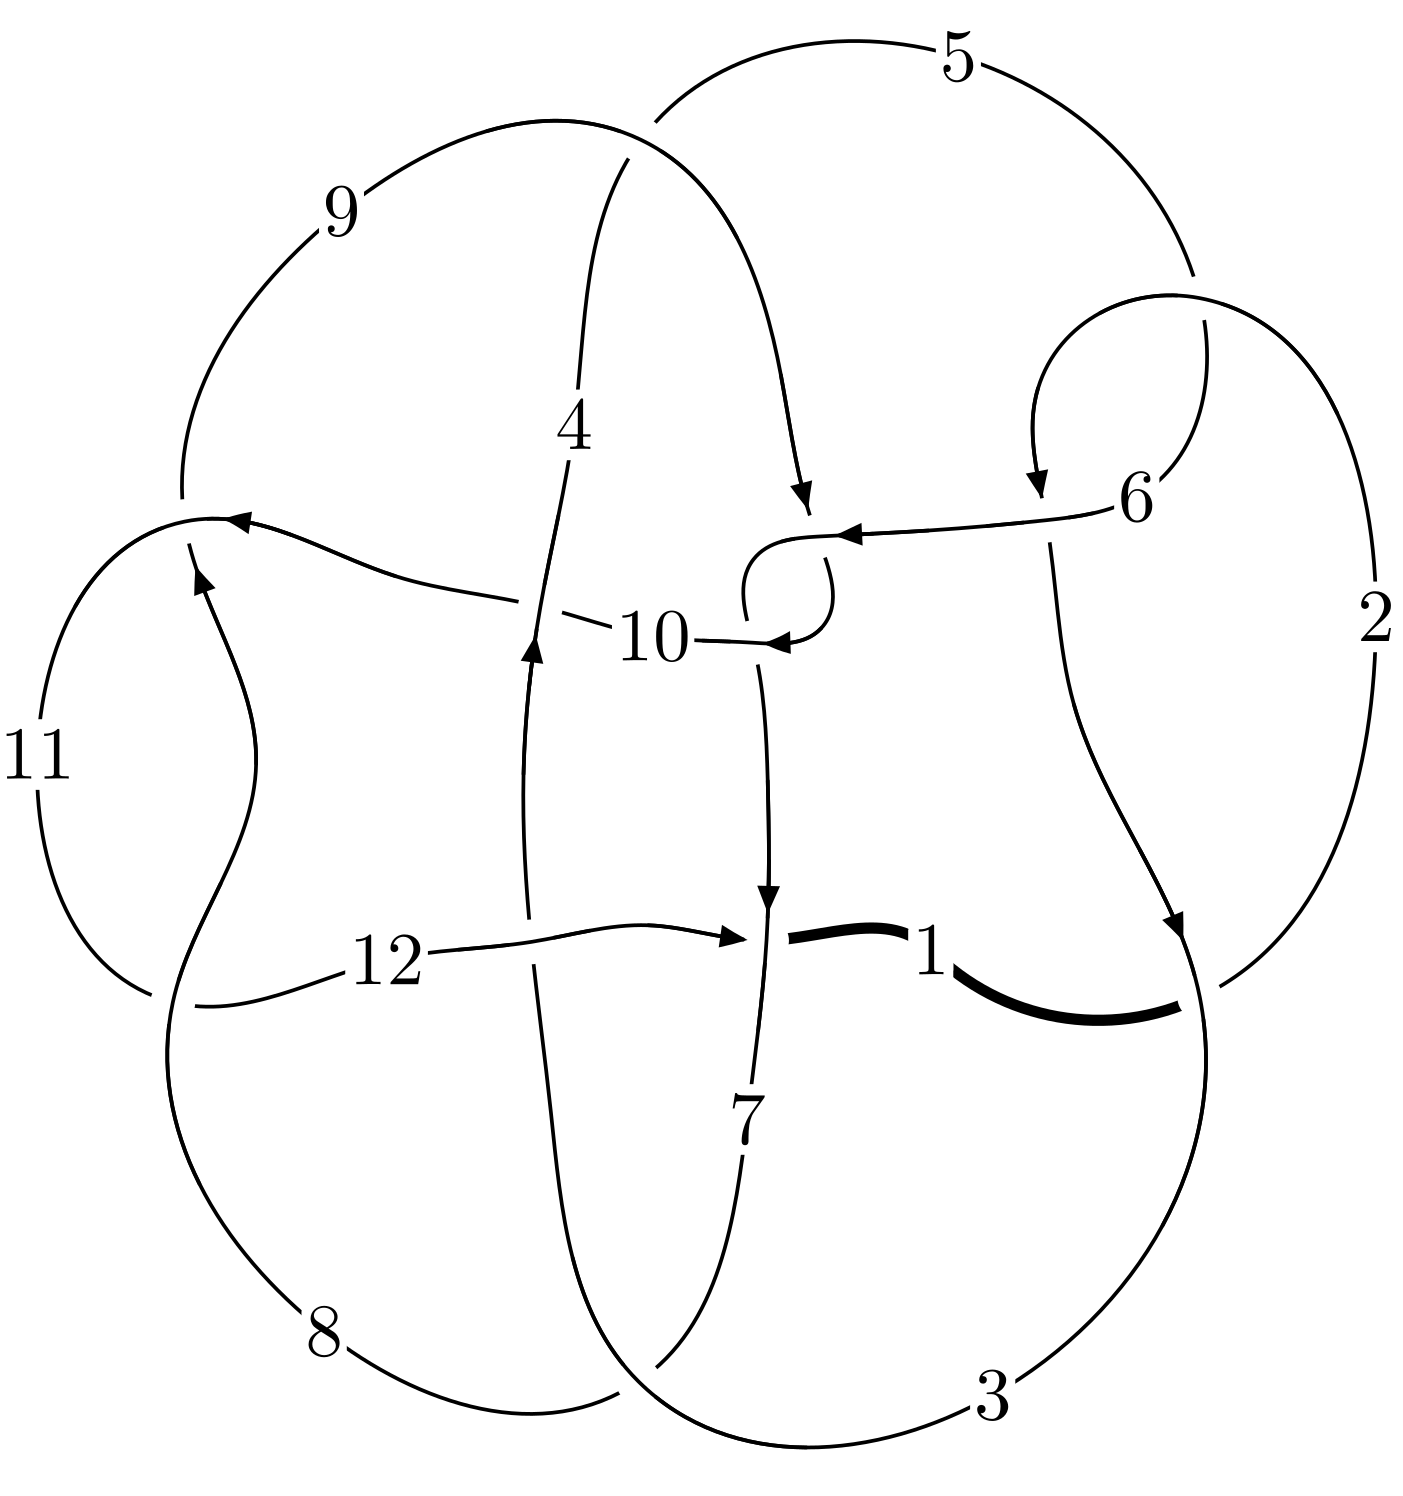
\includegraphics[width=112pt]{../../../GIT/diagram.site/Diagrams/png/2508_12n_0419.png}\\
\ \ \ A knot diagram\footnotemark}&
\allowdisplaybreaks
\textbf{Linearized knot diagam} \\
\cline{2-2}
 &
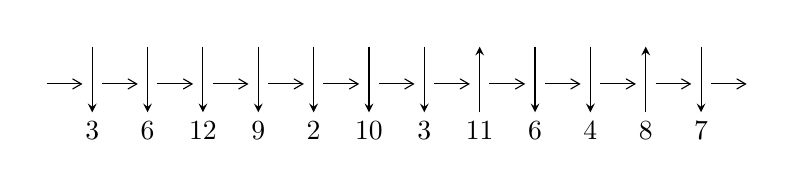
\begin{tikzpicture}[x=20pt, y=17pt]
	% nodes
	\node (C0) at (0, 0) {};
	\node (C1) at (1, 0) {};
	\node (C1U) at (1, +1) {};
	\node (C1D) at (1, -1) {3};

	\node (C2) at (2, 0) {};
	\node (C2U) at (2, +1) {};
	\node (C2D) at (2, -1) {6};

	\node (C3) at (3, 0) {};
	\node (C3U) at (3, +1) {};
	\node (C3D) at (3, -1) {12};

	\node (C4) at (4, 0) {};
	\node (C4U) at (4, +1) {};
	\node (C4D) at (4, -1) {9};

	\node (C5) at (5, 0) {};
	\node (C5U) at (5, +1) {};
	\node (C5D) at (5, -1) {2};

	\node (C6) at (6, 0) {};
	\node (C6U) at (6, +1) {};
	\node (C6D) at (6, -1) {10};

	\node (C7) at (7, 0) {};
	\node (C7U) at (7, +1) {};
	\node (C7D) at (7, -1) {3};

	\node (C8) at (8, 0) {};
	\node (C8U) at (8, +1) {};
	\node (C8D) at (8, -1) {11};

	\node (C9) at (9, 0) {};
	\node (C9U) at (9, +1) {};
	\node (C9D) at (9, -1) {6};

	\node (C10) at (10, 0) {};
	\node (C10U) at (10, +1) {};
	\node (C10D) at (10, -1) {4};

	\node (C11) at (11, 0) {};
	\node (C11U) at (11, +1) {};
	\node (C11D) at (11, -1) {8};

	\node (C12) at (12, 0) {};
	\node (C12U) at (12, +1) {};
	\node (C12D) at (12, -1) {7};
	\node (C13) at (13, 0) {};

	% arrows
	\draw[->,>={angle 60}]
	(C0) edge (C1) (C1) edge (C2) (C2) edge (C3) (C3) edge (C4) (C4) edge (C5) (C5) edge (C6) (C6) edge (C7) (C7) edge (C8) (C8) edge (C9) (C9) edge (C10) (C10) edge (C11) (C11) edge (C12) (C12) edge (C13) ;	\draw[->,>=stealth]
	(C1U) edge (C1D) (C2U) edge (C2D) (C3U) edge (C3D) (C4U) edge (C4D) (C5U) edge (C5D) (C6U) edge (C6D) (C7U) edge (C7D) (C8D) edge (C8U) (C9U) edge (C9D) (C10U) edge (C10D) (C11D) edge (C11U) (C12U) edge (C12D) ;
	\end{tikzpicture} \\
\hhline{~~} \\& 
\textbf{Solving Sequence} \\ \cline{2-2} 
 &
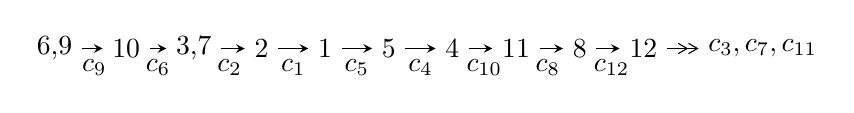
\begin{tikzpicture}[x=23pt, y=7pt]
	% node
	\node (A0) at (-1/8, 0) {6,9};
	\node (A1) at (1, 0) {10};
	\node (A2) at (33/16, 0) {3,7};
	\node (A3) at (25/8, 0) {2};
	\node (A4) at (33/8, 0) {1};
	\node (A5) at (41/8, 0) {5};
	\node (A6) at (49/8, 0) {4};
	\node (A7) at (57/8, 0) {11};
	\node (A8) at (65/8, 0) {8};
	\node (A9) at (73/8, 0) {12};
	\node (C1) at (1/2, -1) {$c_{9}$};
	\node (C2) at (3/2, -1) {$c_{6}$};
	\node (C3) at (21/8, -1) {$c_{2}$};
	\node (C4) at (29/8, -1) {$c_{1}$};
	\node (C5) at (37/8, -1) {$c_{5}$};
	\node (C6) at (45/8, -1) {$c_{4}$};
	\node (C7) at (53/8, -1) {$c_{10}$};
	\node (C8) at (61/8, -1) {$c_{8}$};
	\node (C9) at (69/8, -1) {$c_{12}$};
	\node (A10) at (11, 0) {$c_{3},c_{7},c_{11}$};

	% edge
	\draw[->,>=stealth]	
	(A0) edge (A1) (A1) edge (A2) (A2) edge (A3) (A3) edge (A4) (A4) edge (A5) (A5) edge (A6) (A6) edge (A7) (A7) edge (A8) (A8) edge (A9) ;
	\draw[->>,>={angle 60}]	
	(A9) edge (A10);
\end{tikzpicture} \\ 

\end{tabular} \\

\footnotetext{
The image of knot diagram is generated by the software ``\textbf{Draw programme}" developed by Andrew Bartholomew(\url{http://www.layer8.co.uk/maths/draw/index.htm\#Running-draw}), where we modified some parts for our purpose(\url{https://github.com/CATsTAILs/LinksPainter}).
}\phantom \\ \newline 
\centering \textbf{Ideals for irreducible components\footnotemark of $X_{\text{par}}$} 
 
\begin{align*}
I^u_{1}&=\langle 
1.66310\times10^{40} u^{18}+2.05150\times10^{40} u^{17}+\cdots+1.58940\times10^{42} b+1.51319\times10^{42},\\
\phantom{I^u_{1}}&\phantom{= \langle  }-1.49523\times10^{41} u^{18}-1.67879\times10^{41} u^{17}+\cdots+2.70197\times10^{43} a+4.39022\times10^{43},\\
\phantom{I^u_{1}}&\phantom{= \langle  }u^{19}+2 u^{18}+\cdots+197 u+34\rangle \\
I^u_{2}&=\langle 
-6 u^{11}+17 u^{10}+15 u^9-46 u^8-27 u^7+16 u^6+67 u^5+36 u^4-81 u^3-12 u^2+3 b+33 u-13,\\
\phantom{I^u_{2}}&\phantom{= \langle  }- u^{11}+8 u^9+6 u^8-20 u^7-23 u^6+6 u^5+33 u^4+24 u^3-24 u^2+3 a-13 u+12,\\
\phantom{I^u_{2}}&\phantom{= \langle  }u^{12}-3 u^{11}-2 u^{10}+8 u^9+3 u^8-3 u^7-10 u^6-4 u^5+14 u^4-2 u^3-6 u^2+4 u-1\rangle \\
I^u_{3}&=\langle 
- u^3 b+u^3+b^2+u^2- u-1,\;u^3+a- u,\;u^4- u^2+1\rangle \\
I^u_{4}&=\langle 
b+u-1,\;a- u+1,\;u^2- u+1\rangle \\
\\
\end{align*}
\raggedright * 4 irreducible components of $\dim_{\mathbb{C}}=0$, with total 41 representations.\\
\footnotetext{All coefficients of polynomials are rational numbers. But the coefficients are sometimes approximated in decimal forms when there is not enough margin.}
\newpage
\renewcommand{\arraystretch}{1}
\centering \section*{I. $I^u_{1}= \langle 1.66\times10^{40} u^{18}+2.05\times10^{40} u^{17}+\cdots+1.59\times10^{42} b+1.51\times10^{42},\;-1.50\times10^{41} u^{18}-1.68\times10^{41} u^{17}+\cdots+2.70\times10^{43} a+4.39\times10^{43},\;u^{19}+2 u^{18}+\cdots+197 u+34 \rangle$}
\flushleft \textbf{(i) Arc colorings}\\
\begin{tabular}{m{7pt} m{180pt} m{7pt} m{180pt} }
\flushright $a_{6}=$&$\begin{pmatrix}0\\u\end{pmatrix}$ \\
\flushright $a_{9}=$&$\begin{pmatrix}1\\0\end{pmatrix}$ \\
\flushright $a_{10}=$&$\begin{pmatrix}1\\u^2\end{pmatrix}$ \\
\flushright $a_{3}=$&$\begin{pmatrix}0.00553383 u^{18}+0.00621320 u^{17}+\cdots+4.05205 u-1.62482\\-0.0104638 u^{18}-0.0129074 u^{17}+\cdots-4.49529 u-0.952055\end{pmatrix}$ \\
\flushright $a_{7}=$&$\begin{pmatrix}- u\\- u^3+u\end{pmatrix}$ \\
\flushright $a_{2}=$&$\begin{pmatrix}0.00553383 u^{18}+0.00621320 u^{17}+\cdots+4.05205 u-1.62482\\-0.0124793 u^{18}-0.0173211 u^{17}+\cdots-5.26347 u-1.11711\end{pmatrix}$ \\
\flushright $a_{1}=$&$\begin{pmatrix}-0.0156043 u^{18}-0.0294312 u^{17}+\cdots-5.04992 u-3.27835\\0.00435103 u^{18}+0.00855543 u^{17}+\cdots-2.18420 u-0.489130\end{pmatrix}$ \\
\flushright $a_{5}=$&$\begin{pmatrix}0.0196881 u^{18}+0.0324028 u^{17}+\cdots+5.22408 u+0.287287\\-0.0163849 u^{18}-0.0268543 u^{17}+\cdots-3.04420 u-0.799678\end{pmatrix}$ \\
\flushright $a_{4}=$&$\begin{pmatrix}0.00330322 u^{18}+0.00554852 u^{17}+\cdots+2.17988 u-0.512391\\-0.0163849 u^{18}-0.0268543 u^{17}+\cdots-3.04420 u-0.799678\end{pmatrix}$ \\
\flushright $a_{11}=$&$\begin{pmatrix}0.0271290 u^{18}+0.0462190 u^{17}+\cdots+4.83481 u+2.57786\\0.000739414 u^{18}+0.00488659 u^{17}+\cdots+0.324280 u+0.739169\end{pmatrix}$ \\
\flushright $a_{8}=$&$\begin{pmatrix}-0.00330322 u^{18}-0.00554852 u^{17}+\cdots-2.17988 u+0.512391\\0.0151808 u^{18}+0.0269510 u^{17}+\cdots+2.74012 u+0.653062\end{pmatrix}$ \\
\flushright $a_{12}=$&$\begin{pmatrix}-0.0134032 u^{18}-0.0261459 u^{17}+\cdots-5.10567 u-3.36811\\0.00236078 u^{18}+0.00585106 u^{17}+\cdots-1.98324 u-0.361402\end{pmatrix}$\\&\end{tabular}
\flushleft \textbf{(ii) Obstruction class $= -1$}\\~\\
\flushleft \textbf{(iii) Cusp Shapes $= 0.0105559 u^{18}+0.0127073 u^{17}+\cdots+11.9187 u-12.1302$}\\~\\
\newpage\renewcommand{\arraystretch}{1}
\flushleft \textbf{(iv) u-Polynomials at the component}\newline \\
\begin{tabular}{m{50pt}|m{274pt}}
Crossings & \hspace{64pt}u-Polynomials at each crossing \\
\hline $$\begin{aligned}c_{1}\end{aligned}$$&$\begin{aligned}
&u^{19}+97 u^{18}+\cdots-1941683 u+162409
\end{aligned}$\\
\hline $$\begin{aligned}c_{2},c_{5}\end{aligned}$$&$\begin{aligned}
&u^{19}+3 u^{18}+\cdots-721 u-403
\end{aligned}$\\
\hline $$\begin{aligned}c_{3}\end{aligned}$$&$\begin{aligned}
&u^{19}-5 u^{18}+\cdots-24 u+11
\end{aligned}$\\
\hline $$\begin{aligned}c_{4}\end{aligned}$$&$\begin{aligned}
&u^{19}-5 u^{18}+\cdots+270503 u+65171
\end{aligned}$\\
\hline $$\begin{aligned}c_{6},c_{9}\end{aligned}$$&$\begin{aligned}
&u^{19}+2 u^{18}+\cdots+197 u+34
\end{aligned}$\\
\hline $$\begin{aligned}c_{7}\end{aligned}$$&$\begin{aligned}
&u^{19}-5 u^{18}+\cdots+94 u-421
\end{aligned}$\\
\hline $$\begin{aligned}c_{8},c_{11}\end{aligned}$$&$\begin{aligned}
&u^{19}+4 u^{18}+\cdots+111 u+9
\end{aligned}$\\
\hline $$\begin{aligned}c_{10}\end{aligned}$$&$\begin{aligned}
&u^{19}+u^{18}+\cdots+706 u+167
\end{aligned}$\\
\hline $$\begin{aligned}c_{12}\end{aligned}$$&$\begin{aligned}
&u^{19}+4 u^{18}+\cdots-13967 u-14044
\end{aligned}$\\
\hline
\end{tabular}\\~\\
\newpage\renewcommand{\arraystretch}{1}
\flushleft \textbf{(v) Riley Polynomials at the component}\newline \\
\begin{tabular}{m{50pt}|m{274pt}}
Crossings & \hspace{64pt}Riley Polynomials at each crossing \\
\hline $$\begin{aligned}c_{1}\end{aligned}$$&$\begin{aligned}
&y^{19}-3221 y^{18}+\cdots+5217004770233 y-26376683281
\end{aligned}$\\
\hline $$\begin{aligned}c_{2},c_{5}\end{aligned}$$&$\begin{aligned}
&y^{19}-97 y^{18}+\cdots-1941683 y-162409
\end{aligned}$\\
\hline $$\begin{aligned}c_{3}\end{aligned}$$&$\begin{aligned}
&y^{19}-9 y^{18}+\cdots+1588 y-121
\end{aligned}$\\
\hline $$\begin{aligned}c_{4}\end{aligned}$$&$\begin{aligned}
&y^{19}-193 y^{18}+\cdots+27615258537 y-4247259241
\end{aligned}$\\
\hline $$\begin{aligned}c_{6},c_{9}\end{aligned}$$&$\begin{aligned}
&y^{19}-54 y^{18}+\cdots+33165 y-1156
\end{aligned}$\\
\hline $$\begin{aligned}c_{7}\end{aligned}$$&$\begin{aligned}
&y^{19}-55 y^{18}+\cdots+783476 y-177241
\end{aligned}$\\
\hline $$\begin{aligned}c_{8},c_{11}\end{aligned}$$&$\begin{aligned}
&y^{19}+8 y^{18}+\cdots+4023 y-81
\end{aligned}$\\
\hline $$\begin{aligned}c_{10}\end{aligned}$$&$\begin{aligned}
&y^{19}+y^{18}+\cdots+293694 y-27889
\end{aligned}$\\
\hline $$\begin{aligned}c_{12}\end{aligned}$$&$\begin{aligned}
&y^{19}-210 y^{18}+\cdots+15988001 y-197233936
\end{aligned}$\\
\hline
\end{tabular}\\~\\
\newpage\flushleft \textbf{(vi) Complex Volumes and Cusp Shapes}
$$\begin{array}{c|c|c}  
\text{Solutions to }I^u_{1}& \I (\text{vol} + \sqrt{-1}CS) & \text{Cusp shape}\\
 \hline 
\begin{aligned}
u &= -0.461221 + 0.540098 I \\
a &= -0.329642 + 0.316078 I \\
b &= -0.029910 + 0.572548 I\end{aligned}
 & -1.03982 + 1.81601 I & -6.18544 - 3.90826 I \\ \hline\begin{aligned}
u &= -0.461221 - 0.540098 I \\
a &= -0.329642 - 0.316078 I \\
b &= -0.029910 - 0.572548 I\end{aligned}
 & -1.03982 - 1.81601 I & -6.18544 + 3.90826 I \\ \hline\begin{aligned}
u &= -1.088290 + 0.702970 I \\
a &= -0.517058 - 0.653979 I \\
b &= -1.259640 - 0.053971 I\end{aligned}
 & -1.72336 + 1.68833 I & -7.61757 - 1.84714 I \\ \hline\begin{aligned}
u &= -1.088290 - 0.702970 I \\
a &= -0.517058 + 0.653979 I \\
b &= -1.259640 + 0.053971 I\end{aligned}
 & -1.72336 - 1.68833 I & -7.61757 + 1.84714 I \\ \hline\begin{aligned}
u &= \phantom{-}1.36853 + 0.50280 I \\
a &= -0.383197 + 0.779759 I \\
b &= -1.84064 + 0.23118 I\end{aligned}
 & -8.13748 - 4.76151 I & -14.1488 + 2.3927 I \\ \hline\begin{aligned}
u &= \phantom{-}1.36853 - 0.50280 I \\
a &= -0.383197 - 0.779759 I \\
b &= -1.84064 - 0.23118 I\end{aligned}
 & -8.13748 + 4.76151 I & -14.1488 - 2.3927 I \\ \hline\begin{aligned}
u &= -0.347878 + 0.247156 I \\
a &= -2.26272 - 0.83175 I \\
b &= \phantom{-}0.56233 + 1.35367 I\end{aligned}
 & -3.68506 + 0.25072 I & -15.1444 - 0.1476 I \\ \hline\begin{aligned}
u &= -0.347878 - 0.247156 I \\
a &= -2.26272 + 0.83175 I \\
b &= \phantom{-}0.56233 - 1.35367 I\end{aligned}
 & -3.68506 - 0.25072 I & -15.1444 + 0.1476 I \\ \hline\begin{aligned}
u &= \phantom{-}0.310858 + 0.201294 I \\
a &= \phantom{-}0.06485 + 2.00660 I \\
b &= -2.14079 + 0.42046 I\end{aligned}
 & -3.21447 + 6.05819 I & -7.22138 - 2.86734 I \\ \hline\begin{aligned}
u &= \phantom{-}0.310858 - 0.201294 I \\
a &= \phantom{-}0.06485 - 2.00660 I \\
b &= -2.14079 - 0.42046 I\end{aligned}
 & -3.21447 - 6.05819 I & -7.22138 + 2.86734 I\\
 \hline 
 \end{array}$$\newpage$$\begin{array}{c|c|c}  
\text{Solutions to }I^u_{1}& \I (\text{vol} + \sqrt{-1}CS) & \text{Cusp shape}\\
 \hline 
\begin{aligned}
u &= \phantom{-}0.21322 + 1.62429 I \\
a &= -0.704489 + 0.702997 I \\
b &= \phantom{-}2.62979 - 2.27449 I\end{aligned}
 & \phantom{-}1.70124 + 2.03414 I & -9.92889 - 4.28864 I \\ \hline\begin{aligned}
u &= \phantom{-}0.21322 - 1.62429 I \\
a &= -0.704489 - 0.702997 I \\
b &= \phantom{-}2.62979 + 2.27449 I\end{aligned}
 & \phantom{-}1.70124 - 2.03414 I & -9.92889 + 4.28864 I \\ \hline\begin{aligned}
u &= -0.230182\phantom{ +0.000000I} \\
a &= -1.93660\phantom{ +0.000000I} \\
b &= -0.473485\phantom{ +0.000000I}\end{aligned}
 & -0.715844\phantom{ +0.000000I} & -14.1990\phantom{ +0.000000I} \\ \hline\begin{aligned}
u &= \phantom{-}2.32815\phantom{ +0.000000I} \\
a &= -1.06005\phantom{ +0.000000I} \\
b &= -3.36761\phantom{ +0.000000I}\end{aligned}
 & -18.6560\phantom{ +0.000000I} & -21.4300\phantom{ +0.000000I} \\ \hline\begin{aligned}
u &= -2.39736 + 1.54309 I \\
a &= -1.141170 - 0.008691 I \\
b &= -1.78841 + 8.62679 I\end{aligned}
 & \phantom{-}12.7776 + 11.8645 I & -10.68698 - 4.25583 I \\ \hline\begin{aligned}
u &= -2.39736 - 1.54309 I \\
a &= -1.141170 + 0.008691 I \\
b &= -1.78841 - 8.62679 I\end{aligned}
 & \phantom{-}12.7776 - 11.8645 I & -10.68698 + 4.25583 I \\ \hline\begin{aligned}
u &= -2.64357 + 1.95100 I \\
a &= \phantom{-}1.147970 + 0.222590 I \\
b &= \phantom{-}3.90696 - 11.33980 I\end{aligned}
 & \phantom{-}13.49670 + 2.32138 I & -10.59401 + 0. I\phantom{ +0.000000I} \\ \hline\begin{aligned}
u &= -2.64357 - 1.95100 I \\
a &= \phantom{-}1.147970 - 0.222590 I \\
b &= \phantom{-}3.90696 + 11.33980 I\end{aligned}
 & \phantom{-}13.49670 - 2.32138 I & -10.59401 + 0. I\phantom{ +0.000000I} \\ \hline\begin{aligned}
u &= \phantom{-}5.99343\phantom{ +0.000000I} \\
a &= \phantom{-}1.27698\phantom{ +0.000000I} \\
b &= \phantom{-}43.7617\phantom{ +0.000000I}\end{aligned}
 & \phantom{-}17.1155\phantom{ +0.000000I} & \phantom{-0.000000 } 0\\
 \hline 
 \end{array}$$\newpage\newpage\renewcommand{\arraystretch}{1}
\centering \section*{II. $I^u_{2}= \langle -6 u^{11}+17 u^{10}+\cdots+3 b-13,\;- u^{11}+8 u^9+\cdots+3 a+12,\;u^{12}-3 u^{11}+\cdots+4 u-1 \rangle$}
\flushleft \textbf{(i) Arc colorings}\\
\begin{tabular}{m{7pt} m{180pt} m{7pt} m{180pt} }
\flushright $a_{6}=$&$\begin{pmatrix}0\\u\end{pmatrix}$ \\
\flushright $a_{9}=$&$\begin{pmatrix}1\\0\end{pmatrix}$ \\
\flushright $a_{10}=$&$\begin{pmatrix}1\\u^2\end{pmatrix}$ \\
\flushright $a_{3}=$&$\begin{pmatrix}\frac{1}{3} u^{11}-\frac{8}{3} u^9+\cdots+\frac{13}{3} u-4\\2 u^{11}-\frac{17}{3} u^{10}+\cdots-11 u+\frac{13}{3}\end{pmatrix}$ \\
\flushright $a_{7}=$&$\begin{pmatrix}- u\\- u^3+u\end{pmatrix}$ \\
\flushright $a_{2}=$&$\begin{pmatrix}\frac{1}{3} u^{11}-\frac{8}{3} u^9+\cdots+\frac{13}{3} u-4\\u^{11}-3 u^{10}+\cdots-\frac{22}{3} u+\frac{10}{3}\end{pmatrix}$ \\
\flushright $a_{1}=$&$\begin{pmatrix}\frac{1}{3} u^{11}-\frac{7}{3} u^{10}+\cdots-13 u+7\\-\frac{1}{3} u^{11}+\frac{4}{3} u^{10}+\cdots+\frac{22}{3} u-\frac{1}{3}\end{pmatrix}$ \\
\flushright $a_{5}=$&$\begin{pmatrix}-\frac{2}{3} u^{11}+\frac{1}{3} u^{10}+\cdots-\frac{22}{3} u+6\\\frac{1}{3} u^{11}-\frac{1}{3} u^{10}+\cdots+\frac{13}{3} u-\frac{4}{3}\end{pmatrix}$ \\
\flushright $a_{4}=$&$\begin{pmatrix}-\frac{1}{3} u^{11}+\frac{10}{3} u^9+\cdots-3 u+\frac{14}{3}\\\frac{1}{3} u^{11}-\frac{1}{3} u^{10}+\cdots+\frac{13}{3} u-\frac{4}{3}\end{pmatrix}$ \\
\flushright $a_{11}=$&$\begin{pmatrix}-\frac{8}{3} u^{11}+\frac{22}{3} u^{10}+\cdots+15 u-\frac{7}{3}\\-\frac{4}{3} u^{11}+\frac{11}{3} u^{10}+\cdots+\frac{20}{3} u-\frac{10}{3}\end{pmatrix}$ \\
\flushright $a_{8}=$&$\begin{pmatrix}\frac{1}{3} u^{11}-\frac{10}{3} u^9+\cdots+3 u-\frac{14}{3}\\\frac{4}{3} u^{11}-3 u^{10}+\cdots-\frac{23}{3} u+2\end{pmatrix}$ \\
\flushright $a_{12}=$&$\begin{pmatrix}-\frac{2}{3} u^{11}+\frac{1}{3} u^{10}+\cdots-\frac{25}{3} u+6\\\frac{1}{3} u^{10}- u^9+\cdots+3 u+\frac{1}{3}\end{pmatrix}$\\&\end{tabular}
\flushleft \textbf{(ii) Obstruction class $= 1$}\\~\\
\flushleft \textbf{(iii) Cusp Shapes $= -\frac{46}{3} u^{11}+33 u^{10}+62 u^9-\frac{247}{3} u^8-114 u^7-\frac{91}{3} u^6+\frac{388}{3} u^5+\frac{526}{3} u^4-\frac{304}{3} u^3-\frac{176}{3} u^2+\frac{181}{3} u-\frac{107}{3}$}\\~\\
\newpage\renewcommand{\arraystretch}{1}
\flushleft \textbf{(iv) u-Polynomials at the component}\newline \\
\begin{tabular}{m{50pt}|m{274pt}}
Crossings & \hspace{64pt}u-Polynomials at each crossing \\
\hline $$\begin{aligned}c_{1}\end{aligned}$$&$\begin{aligned}
&u^{12}-10 u^{11}+\cdots+2 u+1
\end{aligned}$\\
\hline $$\begin{aligned}c_{2}\end{aligned}$$&$\begin{aligned}
&u^{12}+8 u^{11}+\cdots-4 u-1
\end{aligned}$\\
\hline $$\begin{aligned}c_{3}\end{aligned}$$&$\begin{aligned}
&u^{12}+3 u^{11}+\cdots-4 u-1
\end{aligned}$\\
\hline $$\begin{aligned}c_{4}\end{aligned}$$&$\begin{aligned}
&u^{12}-3 u^{11}+\cdots-113 u+61
\end{aligned}$\\
\hline $$\begin{aligned}c_{5}\end{aligned}$$&$\begin{aligned}
&u^{12}-8 u^{11}+\cdots+4 u-1
\end{aligned}$\\
\hline $$\begin{aligned}c_{6}\end{aligned}$$&$\begin{aligned}
&u^{12}+3 u^{11}+\cdots-4 u-1
\end{aligned}$\\
\hline $$\begin{aligned}c_{7}\end{aligned}$$&$\begin{aligned}
&u^{12}+3 u^{11}+\cdots-2 u-1
\end{aligned}$\\
\hline $$\begin{aligned}c_{8}\end{aligned}$$&$\begin{aligned}
&u^{12}+3 u^{11}+\cdots+6 u+1
\end{aligned}$\\
\hline $$\begin{aligned}c_{9}\end{aligned}$$&$\begin{aligned}
&u^{12}-3 u^{11}+\cdots+4 u-1
\end{aligned}$\\
\hline $$\begin{aligned}c_{10}\end{aligned}$$&$\begin{aligned}
&u^{12}+u^{11}+u^{10}- u^9-2 u^8-7 u^7-3 u^6-4 u^5+4 u^4- u^3+3 u^2+1
\end{aligned}$\\
\hline $$\begin{aligned}c_{11}\end{aligned}$$&$\begin{aligned}
&u^{12}-3 u^{11}+\cdots-6 u+1
\end{aligned}$\\
\hline $$\begin{aligned}c_{12}\end{aligned}$$&$\begin{aligned}
&u^{12}-7 u^{11}+\cdots-149 u+61
\end{aligned}$\\
\hline
\end{tabular}\\~\\
\newpage\renewcommand{\arraystretch}{1}
\flushleft \textbf{(v) Riley Polynomials at the component}\newline \\
\begin{tabular}{m{50pt}|m{274pt}}
Crossings & \hspace{64pt}Riley Polynomials at each crossing \\
\hline $$\begin{aligned}c_{1}\end{aligned}$$&$\begin{aligned}
&y^{12}-70 y^{11}+\cdots-18 y+1
\end{aligned}$\\
\hline $$\begin{aligned}c_{2},c_{5}\end{aligned}$$&$\begin{aligned}
&y^{12}-10 y^{11}+\cdots+2 y+1
\end{aligned}$\\
\hline $$\begin{aligned}c_{3}\end{aligned}$$&$\begin{aligned}
&y^{12}-3 y^{11}+\cdots-6 y+1
\end{aligned}$\\
\hline $$\begin{aligned}c_{4}\end{aligned}$$&$\begin{aligned}
&y^{12}-11 y^{11}+\cdots+2725 y+3721
\end{aligned}$\\
\hline $$\begin{aligned}c_{6},c_{9}\end{aligned}$$&$\begin{aligned}
&y^{12}-13 y^{11}+\cdots-4 y+1
\end{aligned}$\\
\hline $$\begin{aligned}c_{7}\end{aligned}$$&$\begin{aligned}
&y^{12}-19 y^{11}+\cdots-16 y+1
\end{aligned}$\\
\hline $$\begin{aligned}c_{8},c_{11}\end{aligned}$$&$\begin{aligned}
&y^{12}+3 y^{11}+\cdots-20 y+1
\end{aligned}$\\
\hline $$\begin{aligned}c_{10}\end{aligned}$$&$\begin{aligned}
&y^{12}+y^{11}+\cdots+6 y+1
\end{aligned}$\\
\hline $$\begin{aligned}c_{12}\end{aligned}$$&$\begin{aligned}
&y^{12}-33 y^{11}+\cdots-22201 y+3721
\end{aligned}$\\
\hline
\end{tabular}\\~\\
\newpage\flushleft \textbf{(vi) Complex Volumes and Cusp Shapes}
$$\begin{array}{c|c|c}  
\text{Solutions to }I^u_{2}& \I (\text{vol} + \sqrt{-1}CS) & \text{Cusp shape}\\
 \hline 
\begin{aligned}
u &= -1.059480 + 0.154142 I \\
a &= \phantom{-}0.819599 - 0.608253 I \\
b &= -0.415453 - 0.590193 I\end{aligned}
 & \phantom{-}1.22664 + 3.11362 I & -7.04939 - 7.05690 I \\ \hline\begin{aligned}
u &= -1.059480 - 0.154142 I \\
a &= \phantom{-}0.819599 + 0.608253 I \\
b &= -0.415453 + 0.590193 I\end{aligned}
 & \phantom{-}1.22664 - 3.11362 I & -7.04939 + 7.05690 I \\ \hline\begin{aligned}
u &= -0.457840 + 1.081060 I \\
a &= \phantom{-}0.907598 - 0.603898 I \\
b &= -3.07960 - 0.50765 I\end{aligned}
 & \phantom{-}2.31672 + 1.60638 I & -1.16262 - 0.94623 I \\ \hline\begin{aligned}
u &= -0.457840 - 1.081060 I \\
a &= \phantom{-}0.907598 + 0.603898 I \\
b &= -3.07960 + 0.50765 I\end{aligned}
 & \phantom{-}2.31672 - 1.60638 I & -1.16262 + 0.94623 I \\ \hline\begin{aligned}
u &= -1.24242\phantom{ +0.000000I} \\
a &= -0.422158\phantom{ +0.000000I} \\
b &= \phantom{-}0.0575173\phantom{ +0.000000I}\end{aligned}
 & -3.40775\phantom{ +0.000000I} & -11.1910\phantom{ +0.000000I} \\ \hline\begin{aligned}
u &= \phantom{-}0.646031 + 0.179003 I \\
a &= -0.948613 - 0.380726 I \\
b &= \phantom{-}2.25048 + 0.18881 I\end{aligned}
 & -3.62882 - 6.45766 I & -17.3073 + 12.6531 I \\ \hline\begin{aligned}
u &= \phantom{-}0.646031 - 0.179003 I \\
a &= -0.948613 + 0.380726 I \\
b &= \phantom{-}2.25048 - 0.18881 I\end{aligned}
 & -3.62882 + 6.45766 I & -17.3073 - 12.6531 I \\ \hline\begin{aligned}
u &= \phantom{-}1.45298 + 0.05285 I \\
a &= -0.107356 - 0.338014 I \\
b &= -0.694805 - 0.843286 I\end{aligned}
 & -7.20322 - 5.60855 I & -9.98455 + 5.57082 I \\ \hline\begin{aligned}
u &= \phantom{-}1.45298 - 0.05285 I \\
a &= -0.107356 + 0.338014 I \\
b &= -0.694805 + 0.843286 I\end{aligned}
 & -7.20322 + 5.60855 I & -9.98455 - 5.57082 I \\ \hline\begin{aligned}
u &= \phantom{-}0.285356 + 0.363826 I \\
a &= -1.91901 + 3.12576 I \\
b &= -0.84108 - 1.29227 I\end{aligned}
 & -8.23832 - 3.21911 I & -14.7748 - 0.6369 I\\
 \hline 
 \end{array}$$\newpage$$\begin{array}{c|c|c}  
\text{Solutions to }I^u_{2}& \I (\text{vol} + \sqrt{-1}CS) & \text{Cusp shape}\\
 \hline 
\begin{aligned}
u &= \phantom{-}0.285356 - 0.363826 I \\
a &= -1.91901 - 3.12576 I \\
b &= -0.84108 + 1.29227 I\end{aligned}
 & -8.23832 + 3.21911 I & -14.7748 + 0.6369 I \\ \hline\begin{aligned}
u &= \phantom{-}2.50831\phantom{ +0.000000I} \\
a &= -1.08227\phantom{ +0.000000I} \\
b &= -4.49661\phantom{ +0.000000I}\end{aligned}
 & -18.1761\phantom{ +0.000000I} & -4.25130\phantom{ +0.000000I}\\
 \hline 
 \end{array}$$\newpage\newpage\renewcommand{\arraystretch}{1}
\centering \section*{III. $I^u_{3}= \langle - u^3 b+u^3+b^2+u^2- u-1,\;u^3+a- u,\;u^4- u^2+1 \rangle$}
\flushleft \textbf{(i) Arc colorings}\\
\begin{tabular}{m{7pt} m{180pt} m{7pt} m{180pt} }
\flushright $a_{6}=$&$\begin{pmatrix}0\\u\end{pmatrix}$ \\
\flushright $a_{9}=$&$\begin{pmatrix}1\\0\end{pmatrix}$ \\
\flushright $a_{10}=$&$\begin{pmatrix}1\\u^2\end{pmatrix}$ \\
\flushright $a_{3}=$&$\begin{pmatrix}- u^3+u\\b\end{pmatrix}$ \\
\flushright $a_{7}=$&$\begin{pmatrix}- u\\- u^3+u\end{pmatrix}$ \\
\flushright $a_{2}=$&$\begin{pmatrix}- u^3+u\\b- u\end{pmatrix}$ \\
\flushright $a_{1}=$&$\begin{pmatrix}0\\- u\end{pmatrix}$ \\
\flushright $a_{5}=$&$\begin{pmatrix}- u^3+u\\b\end{pmatrix}$ \\
\flushright $a_{4}=$&$\begin{pmatrix}- u^3+b+u\\b\end{pmatrix}$ \\
\flushright $a_{11}=$&$\begin{pmatrix}- u^3 b- u^3- u^2\\- u^3\end{pmatrix}$ \\
\flushright $a_{8}=$&$\begin{pmatrix}u^3- b- u\\-1\end{pmatrix}$ \\
\flushright $a_{12}=$&$\begin{pmatrix}- u^3\\0\end{pmatrix}$\\&\end{tabular}
\flushleft \textbf{(ii) Obstruction class $= 1$}\\~\\
\flushleft \textbf{(iii) Cusp Shapes $= 4 u^2-16$}\\~\\
\newpage\renewcommand{\arraystretch}{1}
\flushleft \textbf{(iv) u-Polynomials at the component}\newline \\
\begin{tabular}{m{50pt}|m{274pt}}
Crossings & \hspace{64pt}u-Polynomials at each crossing \\
\hline $$\begin{aligned}c_{1},c_{2}\end{aligned}$$&$\begin{aligned}
&(u-1)^8
\end{aligned}$\\
\hline $$\begin{aligned}c_{3}\end{aligned}$$&$\begin{aligned}
&u^8+4 u^7+8 u^6+10 u^5+9 u^4+6 u^3-2 u+1
\end{aligned}$\\
\hline $$\begin{aligned}c_{4}\end{aligned}$$&$\begin{aligned}
&u^8+2 u^5+u^4+6 u^3+4 u^2-2 u+1
\end{aligned}$\\
\hline $$\begin{aligned}c_{5}\end{aligned}$$&$\begin{aligned}
&(u+1)^8
\end{aligned}$\\
\hline $$\begin{aligned}c_{6},c_{9}\end{aligned}$$&$\begin{aligned}
&(u^4- u^2+1)^2
\end{aligned}$\\
\hline $$\begin{aligned}c_{7}\end{aligned}$$&$\begin{aligned}
&u^8+2 u^7- u^6-4 u^5+6 u^3+3 u^2-4 u+1
\end{aligned}$\\
\hline $$\begin{aligned}c_{8},c_{11}\end{aligned}$$&$\begin{aligned}
&(u^2+1)^4
\end{aligned}$\\
\hline $$\begin{aligned}c_{10}\end{aligned}$$&$\begin{aligned}
&u^8+3 u^6-2 u^5+4 u^4+7 u^2+2 u+1
\end{aligned}$\\
\hline $$\begin{aligned}c_{12}\end{aligned}$$&$\begin{aligned}
&(u^2+u+1)^4
\end{aligned}$\\
\hline
\end{tabular}\\~\\
\newpage\renewcommand{\arraystretch}{1}
\flushleft \textbf{(v) Riley Polynomials at the component}\newline \\
\begin{tabular}{m{50pt}|m{274pt}}
Crossings & \hspace{64pt}Riley Polynomials at each crossing \\
\hline $$\begin{aligned}c_{1},c_{2},c_{5}\end{aligned}$$&$\begin{aligned}
&(y-1)^8
\end{aligned}$\\
\hline $$\begin{aligned}c_{3}\end{aligned}$$&$\begin{aligned}
&y^8+2 y^6-4 y^5-21 y^4+20 y^3+42 y^2-4 y+1
\end{aligned}$\\
\hline $$\begin{aligned}c_{4}\end{aligned}$$&$\begin{aligned}
&y^8+2 y^6+4 y^5-21 y^4-20 y^3+42 y^2+4 y+1
\end{aligned}$\\
\hline $$\begin{aligned}c_{6},c_{9}\end{aligned}$$&$\begin{aligned}
&(y^2- y+1)^4
\end{aligned}$\\
\hline $$\begin{aligned}c_{7}\end{aligned}$$&$\begin{aligned}
&y^8-6 y^7+17 y^6-34 y^5+60 y^4-70 y^3+57 y^2-10 y+1
\end{aligned}$\\
\hline $$\begin{aligned}c_{8},c_{11}\end{aligned}$$&$\begin{aligned}
&(y+1)^8
\end{aligned}$\\
\hline $$\begin{aligned}c_{10}\end{aligned}$$&$\begin{aligned}
&y^8+6 y^7+17 y^6+34 y^5+60 y^4+70 y^3+57 y^2+10 y+1
\end{aligned}$\\
\hline $$\begin{aligned}c_{12}\end{aligned}$$&$\begin{aligned}
&(y^2+y+1)^4
\end{aligned}$\\
\hline
\end{tabular}\\~\\
\newpage\flushleft \textbf{(vi) Complex Volumes and Cusp Shapes}
$$\begin{array}{c|c|c}  
\text{Solutions to }I^u_{3}& \I (\text{vol} + \sqrt{-1}CS) & \text{Cusp shape}\\
 \hline 
\begin{aligned}
u &= \phantom{-}0.866025 + 0.500000 I \\
a &= \phantom{-}0.866025 - 0.500000 I \\
b &= \phantom{-}1.200000 - 0.069179 I\end{aligned}
 & -3.28987 - 2.02988 I & -14.0000 + 3.4641 I \\ \hline\begin{aligned}
u &= \phantom{-}0.866025 + 0.500000 I \\
a &= \phantom{-}0.866025 - 0.500000 I \\
b &= -1.20000 + 1.06918 I\end{aligned}
 & -3.28987 - 2.02988 I & -14.0000 + 3.4641 I \\ \hline\begin{aligned}
u &= \phantom{-}0.866025 - 0.500000 I \\
a &= \phantom{-}0.866025 + 0.500000 I \\
b &= \phantom{-}1.200000 + 0.069179 I\end{aligned}
 & -3.28987 + 2.02988 I & -14.0000 - 3.4641 I \\ \hline\begin{aligned}
u &= \phantom{-}0.866025 - 0.500000 I \\
a &= \phantom{-}0.866025 + 0.500000 I \\
b &= -1.20000 - 1.06918 I\end{aligned}
 & -3.28987 + 2.02988 I & -14.0000 - 3.4641 I \\ \hline\begin{aligned}
u &= -0.866025 + 0.500000 I \\
a &= -0.866025 - 0.500000 I \\
b &= \phantom{-}0.224207 + 1.316270 I\end{aligned}
 & -3.28987 + 2.02988 I & -14.0000 - 3.4641 I \\ \hline\begin{aligned}
u &= -0.866025 + 0.500000 I \\
a &= -0.866025 - 0.500000 I \\
b &= -0.224207 - 0.316268 I\end{aligned}
 & -3.28987 + 2.02988 I & -14.0000 - 3.4641 I \\ \hline\begin{aligned}
u &= -0.866025 - 0.500000 I \\
a &= -0.866025 + 0.500000 I \\
b &= \phantom{-}0.224207 - 1.316270 I\end{aligned}
 & -3.28987 - 2.02988 I & -14.0000 + 3.4641 I \\ \hline\begin{aligned}
u &= -0.866025 - 0.500000 I \\
a &= -0.866025 + 0.500000 I \\
b &= -0.224207 + 0.316268 I\end{aligned}
 & -3.28987 - 2.02988 I & -14.0000 + 3.4641 I\\
 \hline 
 \end{array}$$\newpage\newpage\renewcommand{\arraystretch}{1}
\centering \section*{IV. $I^u_{4}= \langle b+u-1,\;a- u+1,\;u^2- u+1 \rangle$}
\flushleft \textbf{(i) Arc colorings}\\
\begin{tabular}{m{7pt} m{180pt} m{7pt} m{180pt} }
\flushright $a_{6}=$&$\begin{pmatrix}0\\u\end{pmatrix}$ \\
\flushright $a_{9}=$&$\begin{pmatrix}1\\0\end{pmatrix}$ \\
\flushright $a_{10}=$&$\begin{pmatrix}1\\u-1\end{pmatrix}$ \\
\flushright $a_{3}=$&$\begin{pmatrix}u-1\\- u+1\end{pmatrix}$ \\
\flushright $a_{7}=$&$\begin{pmatrix}- u\\u+1\end{pmatrix}$ \\
\flushright $a_{2}=$&$\begin{pmatrix}u-1\\1\end{pmatrix}$ \\
\flushright $a_{1}=$&$\begin{pmatrix}0\\u\end{pmatrix}$ \\
\flushright $a_{5}=$&$\begin{pmatrix}- u+1\\u-1\end{pmatrix}$ \\
\flushright $a_{4}=$&$\begin{pmatrix}0\\u-1\end{pmatrix}$ \\
\flushright $a_{11}=$&$\begin{pmatrix}1\\-1\end{pmatrix}$ \\
\flushright $a_{8}=$&$\begin{pmatrix}0\\1\end{pmatrix}$ \\
\flushright $a_{12}=$&$\begin{pmatrix}-1\\2\end{pmatrix}$\\&\end{tabular}
\flushleft \textbf{(ii) Obstruction class $= -1$}\\~\\
\flushleft \textbf{(iii) Cusp Shapes $= -4 u-4$}\\~\\
\newpage\renewcommand{\arraystretch}{1}
\flushleft \textbf{(iv) u-Polynomials at the component}\newline \\
\begin{tabular}{m{50pt}|m{274pt}}
Crossings & \hspace{64pt}u-Polynomials at each crossing \\
\hline $$\begin{aligned}c_{1}\end{aligned}$$&$\begin{aligned}
&(u+1)^2
\end{aligned}$\\
\hline $$\begin{aligned}c_{2},c_{5},c_{8}\\c_{11}\end{aligned}$$&$\begin{aligned}
&(u-1)^2
\end{aligned}$\\
\hline $$\begin{aligned}c_{3},c_{4},c_{10}\end{aligned}$$&$\begin{aligned}
&u^2+u+1
\end{aligned}$\\
\hline $$\begin{aligned}c_{6},c_{7},c_{9}\\c_{12}\end{aligned}$$&$\begin{aligned}
&u^2- u+1
\end{aligned}$\\
\hline
\end{tabular}\\~\\
\newpage\renewcommand{\arraystretch}{1}
\flushleft \textbf{(v) Riley Polynomials at the component}\newline \\
\begin{tabular}{m{50pt}|m{274pt}}
Crossings & \hspace{64pt}Riley Polynomials at each crossing \\
\hline $$\begin{aligned}c_{1},c_{2},c_{5}\\c_{8},c_{11}\end{aligned}$$&$\begin{aligned}
&(y-1)^2
\end{aligned}$\\
\hline $$\begin{aligned}c_{3},c_{4},c_{6}\\c_{7},c_{9},c_{10}\\c_{12}\end{aligned}$$&$\begin{aligned}
&y^2+y+1
\end{aligned}$\\
\hline
\end{tabular}\\~\\
\newpage\flushleft \textbf{(vi) Complex Volumes and Cusp Shapes}
$$\begin{array}{c|c|c}  
\text{Solutions to }I^u_{4}& \I (\text{vol} + \sqrt{-1}CS) & \text{Cusp shape}\\
 \hline 
\begin{aligned}
u &= \phantom{-}0.500000 + 0.866025 I \\
a &= -0.500000 + 0.866025 I \\
b &= \phantom{-}0.500000 - 0.866025 I\end{aligned}
 & \phantom{-}1.64493 + 2.02988 I & -6.00000 - 3.46410 I \\ \hline\begin{aligned}
u &= \phantom{-}0.500000 - 0.866025 I \\
a &= -0.500000 - 0.866025 I \\
b &= \phantom{-}0.500000 + 0.866025 I\end{aligned}
 & \phantom{-}1.64493 - 2.02988 I & -6.00000 + 3.46410 I\\
 \hline 
 \end{array}$$\newpage
\newpage\renewcommand{\arraystretch}{1}
\centering \section*{ V. u-Polynomials}
\begin{tabular}{m{50pt}|m{274pt}}
Crossings & \hspace{64pt}u-Polynomials at each crossing \\
\hline $$\begin{aligned}c_{1}\end{aligned}$$&$\begin{aligned}
&((u-1)^8)(u+1)^2(u^{12}-10 u^{11}+\cdots+2 u+1)\\
&\cdot(u^{19}+97 u^{18}+\cdots-1941683 u+162409)
\end{aligned}$\\
\hline $$\begin{aligned}c_{2}\end{aligned}$$&$\begin{aligned}
&((u-1)^{10})(u^{12}+8 u^{11}+\cdots-4 u-1)(u^{19}+3 u^{18}+\cdots-721 u-403)
\end{aligned}$\\
\hline $$\begin{aligned}c_{3}\end{aligned}$$&$\begin{aligned}
&(u^2+u+1)(u^8+4 u^7+8 u^6+10 u^5+9 u^4+6 u^3-2 u+1)\\
&\cdot(u^{12}+3 u^{11}+\cdots-4 u-1)(u^{19}-5 u^{18}+\cdots-24 u+11)
\end{aligned}$\\
\hline $$\begin{aligned}c_{4}\end{aligned}$$&$\begin{aligned}
&(u^2+u+1)(u^8+2 u^5+u^4+6 u^3+4 u^2-2 u+1)\\
&\cdot(u^{12}-3 u^{11}+\cdots-113 u+61)(u^{19}-5 u^{18}+\cdots+270503 u+65171)
\end{aligned}$\\
\hline $$\begin{aligned}c_{5}\end{aligned}$$&$\begin{aligned}
&((u-1)^2)(u+1)^8(u^{12}-8 u^{11}+\cdots+4 u-1)\\
&\cdot(u^{19}+3 u^{18}+\cdots-721 u-403)
\end{aligned}$\\
\hline $$\begin{aligned}c_{6}\end{aligned}$$&$\begin{aligned}
&(u^2- u+1)(u^4- u^2+1)^2(u^{12}+3 u^{11}+\cdots-4 u-1)\\
&\cdot(u^{19}+2 u^{18}+\cdots+197 u+34)
\end{aligned}$\\
\hline $$\begin{aligned}c_{7}\end{aligned}$$&$\begin{aligned}
&(u^2- u+1)(u^8+2 u^7- u^6-4 u^5+6 u^3+3 u^2-4 u+1)\\
&\cdot(u^{12}+3 u^{11}+\cdots-2 u-1)(u^{19}-5 u^{18}+\cdots+94 u-421)
\end{aligned}$\\
\hline $$\begin{aligned}c_{8}\end{aligned}$$&$\begin{aligned}
&((u-1)^2)(u^2+1)^4(u^{12}+3 u^{11}+\cdots+6 u+1)\\
&\cdot(u^{19}+4 u^{18}+\cdots+111 u+9)
\end{aligned}$\\
\hline $$\begin{aligned}c_{9}\end{aligned}$$&$\begin{aligned}
&(u^2- u+1)(u^4- u^2+1)^2(u^{12}-3 u^{11}+\cdots+4 u-1)\\
&\cdot(u^{19}+2 u^{18}+\cdots+197 u+34)
\end{aligned}$\\
\hline $$\begin{aligned}c_{10}\end{aligned}$$&$\begin{aligned}
&(u^2+u+1)(u^8+3 u^6-2 u^5+4 u^4+7 u^2+2 u+1)\\
&\cdot(u^{12}+u^{11}+u^{10}- u^9-2 u^8-7 u^7-3 u^6-4 u^5+4 u^4- u^3+3 u^2+1)\\
&\cdot(u^{19}+u^{18}+\cdots+706 u+167)
\end{aligned}$\\
\hline $$\begin{aligned}c_{11}\end{aligned}$$&$\begin{aligned}
&((u-1)^2)(u^2+1)^4(u^{12}-3 u^{11}+\cdots-6 u+1)\\
&\cdot(u^{19}+4 u^{18}+\cdots+111 u+9)
\end{aligned}$\\
\hline $$\begin{aligned}c_{12}\end{aligned}$$&$\begin{aligned}
&(u^2- u+1)(u^2+u+1)^4(u^{12}-7 u^{11}+\cdots-149 u+61)\\
&\cdot(u^{19}+4 u^{18}+\cdots-13967 u-14044)
\end{aligned}$\\
\hline
\end{tabular}\newpage\renewcommand{\arraystretch}{1}
\centering \section*{ VI. Riley Polynomials}
\begin{tabular}{m{50pt}|m{274pt}}
Crossings & \hspace{64pt}Riley Polynomials at each crossing \\
\hline $$\begin{aligned}c_{1}\end{aligned}$$&$\begin{aligned}
&((y-1)^{10})(y^{12}-70 y^{11}+\cdots-18 y+1)\\
&\cdot(y^{19}-3221 y^{18}+\cdots+5217004770233 y-26376683281)
\end{aligned}$\\
\hline $$\begin{aligned}c_{2},c_{5}\end{aligned}$$&$\begin{aligned}
&((y-1)^{10})(y^{12}-10 y^{11}+\cdots+2 y+1)\\
&\cdot(y^{19}-97 y^{18}+\cdots-1941683 y-162409)
\end{aligned}$\\
\hline $$\begin{aligned}c_{3}\end{aligned}$$&$\begin{aligned}
&(y^2+y+1)(y^8+2 y^6-4 y^5-21 y^4+20 y^3+42 y^2-4 y+1)\\
&\cdot(y^{12}-3 y^{11}+\cdots-6 y+1)(y^{19}-9 y^{18}+\cdots+1588 y-121)
\end{aligned}$\\
\hline $$\begin{aligned}c_{4}\end{aligned}$$&$\begin{aligned}
&(y^2+y+1)(y^8+2 y^6+4 y^5-21 y^4-20 y^3+42 y^2+4 y+1)\\
&\cdot(y^{12}-11 y^{11}+\cdots+2725 y+3721)\\
&\cdot(y^{19}-193 y^{18}+\cdots+27615258537 y-4247259241)
\end{aligned}$\\
\hline $$\begin{aligned}c_{6},c_{9}\end{aligned}$$&$\begin{aligned}
&((y^2- y+1)^4)(y^2+y+1)(y^{12}-13 y^{11}+\cdots-4 y+1)\\
&\cdot(y^{19}-54 y^{18}+\cdots+33165 y-1156)
\end{aligned}$\\
\hline $$\begin{aligned}c_{7}\end{aligned}$$&$\begin{aligned}
&(y^2+y+1)(y^8-6 y^7+\cdots-10 y+1)\\
&\cdot(y^{12}-19 y^{11}+\cdots-16 y+1)(y^{19}-55 y^{18}+\cdots+783476 y-177241)
\end{aligned}$\\
\hline $$\begin{aligned}c_{8},c_{11}\end{aligned}$$&$\begin{aligned}
&((y-1)^2)(y+1)^8(y^{12}+3 y^{11}+\cdots-20 y+1)\\
&\cdot(y^{19}+8 y^{18}+\cdots+4023 y-81)
\end{aligned}$\\
\hline $$\begin{aligned}c_{10}\end{aligned}$$&$\begin{aligned}
&(y^2+y+1)(y^8+6 y^7+\cdots+10 y+1)\\
&\cdot(y^{12}+y^{11}+\cdots+6 y+1)(y^{19}+y^{18}+\cdots+293694 y-27889)
\end{aligned}$\\
\hline $$\begin{aligned}c_{12}\end{aligned}$$&$\begin{aligned}
&((y^2+y+1)^5)(y^{12}-33 y^{11}+\cdots-22201 y+3721)\\
&\cdot(y^{19}-210 y^{18}+\cdots+15988001 y-197233936)
\end{aligned}$\\
\hline
\end{tabular}
\vskip 2pc
\end{document}